\documentclass [xcolor=svgnames, t] {beamer}
\usepackage[utf8]{inputenc}
\usepackage{booktabs, comment} 
\usepackage[absolute, overlay]{textpos}
\usepackage{pgfpages}
\usepackage[font=footnotesize]{caption}

\setbeamercolor{author in head/foot}{bg=darkcyan}
\setbeamertemplate{page number in head/foot}{}
\usepackage{csquotes}

\usepackage{amsmath}
\usepackage[makeroom]{cancel}

\usepackage{textpos}

\usepackage{tikz}

\usetheme{Madrid}
\definecolor{darkcyan}{RGB}{0, 139, 139}
\usecolortheme[named=darkcyan]{structure}
\usepackage{tikz}

\usepackage{pgfplots}
\pgfplotsset{width=12cm, height=7cm}
\title[Lexical Analysis]{Lexical Analysis}
\subtitle{C Language}
\author[Project 1]{Reyner Marxell Arias Muñoz, Kenneth Ibarra Vargas, David Benavides Naranjo}
\institute[]{Project 1, Compilers and Interpreters course, I 2022 Semester}
\date{\today}

\begin{document}
\begin{frame}
\maketitle
\end{frame}

\begin{frame}{Scanning}
Since the source file has include and define directives, the preprocessor previously applied each of them correctly so that the scanner receives only a temporary input file.
\\Afterwards, the scanner goes through the temporary file returning the tokens one by one and in order, according to the parsed source program. In c there are tokens of different types such as operators, identifiers, literals, reserved words and separator characters.
\\Any character not belonging to the c lexicon that can be parsed is returned as a lexical error.\\
\begin{figure}
\centering

\includegraphics[scale = 0.14]{Scanner.png}
\end{figure}
\end{frame}

\begin{frame}{FLEX}
The scanner is a lex file, which are comprised of three sections:
\begin{itemize}
\item The Definition Section: This sections is made up of several regular expressions that act as global declarations that may be used in the next section.
\item The Rules Section: This section uses the global declarations of the previous section to define what actions must be taken when a specific regular expression is found.
\item The Code Section: This section is attached at the end of the lex output file and may contain any code written and executed by the C code, due to lex usually being paired with yacc. \\
\end{itemize}
\end{frame}

\begin{frame}{Tokens}
\begin{itemize}
\color{OrangeRed}
\item \emph{Operators}
\color{purple}
{\fontfamily{qbk} \selectfont \item Intliterals}
\color{Turquoise}
{\fontfamily{qbk} \selectfont \item \textbf{Floatliterals}}
\color{CadetBlue}
{\fontfamily{qbk} \selectfont \item \underline{\emph{\textbf{Doubleliteral}}}}
\color{Violet}
{\fontfamily{lmdh} \selectfont \item \emph{Charliteral}}
\color{ForestGreen}
{\fontfamily{lmdh} \selectfont \item \textbf{Stringliteral}}
\color{olive}
\item \underline{\textbf{Reserved Words}}
\color{Black}
\item \textbf{Separator characters}
\color{blue}
\item Identifiers
\color{Pink}
{\fontfamily{ptf} \selectfont \item \underline{Errors}}
\end{itemize}
\end{frame}
\begin{frame}{Font Lines}
\color{olive}
\textbf{\underline{int}} 
\color{blue}
test 
\color{Black}
\textbf{(} 
\color{Black}
\textbf{)} 
\color{Black}
\textbf{\{} 
\\\color{blue}
printf 
\color{Black}
\textbf{(} 
\color{ForestGreen}
{\fontfamily{lmdh} \selectfont \textbf{"\%d"}} 
\color{Black}
\textbf{,} 
\color{purple}
{\fontfamily{qbk} \selectfont 1} 
\color{Black}
\textbf{)} 
\color{Black}
\textbf{;} 
\\\color{Black}
\textbf{\}} 
\\\color{olive}
\textbf{\underline{int}} 
\color{blue}
cinco 
\color{OrangeRed}
\emph{=} 
\color{purple}
{\fontfamily{qbk} \selectfont 5} 
\color{Black}
\textbf{;} 
\\\color{olive}
\textbf{\underline{int}} 
\color{blue}
main 
\color{Black}
\textbf{(} 
\color{Black}
\textbf{)} 
\color{Black}
\textbf{\{} 
\\\color{olive}
\textbf{\underline{int}} 
\color{blue}
t 
\color{OrangeRed}
\emph{=} 
\color{purple}
{\fontfamily{qbk} \selectfont 100301} 
\color{Black}
\textbf{;} 
\\\color{olive}
\textbf{\underline{int}} 
\color{blue}
r 
\color{OrangeRed}
\emph{=} 
\color{Pink}
{\fontfamily{ptf} \selectfont \underline{1hola}} 
\color{Black}
\textbf{(} 
\color{Black}
\textbf{)} 
\color{Black}
\textbf{;} 
\\\color{olive}
\textbf{\underline{char}} 
\color{blue}
f 
\color{Black}
\textbf{[} 
\color{purple}
{\fontfamily{qbk} \selectfont 10} 
\color{Black}
\textbf{]} 
\color{OrangeRed}
\emph{=} 
\color{OrangeRed}
\emph{"} 
\color{Black}
\textbf{;} 
\\\color{olive}
\textbf{\underline{int}} 
\color{blue}
v 
\color{OrangeRed}
\emph{=} 
\color{purple}
{\fontfamily{qbk} \selectfont 1} 
\color{Black}
\textbf{;} 
\\\color{olive}
\textbf{\underline{double}} 
\color{blue}
r 
\color{OrangeRed}
\emph{=} 
\color{CadetBlue}
{\fontfamily{qbk} \selectfont \textbf{\underline{\emph{2.435e2}}}} 
\color{Black}
\textbf{;} 
\\\color{olive}
\textbf{\underline{char}} 
\color{blue}
r 
\color{OrangeRed}
\emph{=} 
\color{Violet}
{\fontfamily{lmdh} \selectfont \emph{'y'}} 
\color{Black}
\textbf{;} 
\\\color{blue}
printf 
\color{Black}
\textbf{(} 
\color{ForestGreen}
{\fontfamily{lmdh} \selectfont \textbf{"\%s"}} 
\color{Black}
\textbf{,} 
\color{blue}
f 
\color{Black}
\textbf{)} 
\color{Black}
\textbf{;} 
\\\color{Black}
\textbf{\}} 
\\\color{olive}
\textbf{\underline{int}} 
\color{blue}
main 
\color{Black}
\textbf{(} 
\color{Black}
\textbf{)} 
\color{Black}
\textbf{\{} 
\\\color{olive}
\textbf{\underline{int}} 
\color{blue}
t 
\color{OrangeRed}
\emph{=} 
\color{purple}
{\fontfamily{qbk} \selectfont 100301} 
\color{Black}
\textbf{;} 
\\\color{olive}
\textbf{\underline{int}} 
\color{blue}
r 
\color{OrangeRed}
\emph{=} 
\color{blue}
hola 
\color{Black}
\textbf{(} 
\color{Black}
\textbf{)} 
\color{Black}
\textbf{;} 
\\\end{frame}
\begin{frame}{Font Lines}
\color{olive}
\textbf{\underline{char}} 
\color{blue}
f 
\color{Black}
\textbf{[} 
\color{purple}
{\fontfamily{qbk} \selectfont 10} 
\color{Black}
\textbf{]} 
\color{OrangeRed}
\emph{=} 
\color{OrangeRed}
\emph{"} 
\color{Black}
\textbf{;} 
\\\color{olive}
\textbf{\underline{int}} 
\color{blue}
v 
\color{OrangeRed}
\emph{=} 
\color{purple}
{\fontfamily{qbk} \selectfont 1} 
\color{Black}
\textbf{;} 
\\\color{olive}
\textbf{\underline{double}} 
\color{blue}
r 
\color{OrangeRed}
\emph{=} 
\color{CadetBlue}
{\fontfamily{qbk} \selectfont \textbf{\underline{\emph{2.435e2}}}} 
\color{Black}
\textbf{;} 
\\\color{olive}
\textbf{\underline{char}} 
\color{blue}
r 
\color{OrangeRed}
\emph{=} 
\color{Violet}
{\fontfamily{lmdh} \selectfont \emph{'y'}} 
\color{Black}
\textbf{;} 
\\\color{blue}
printf 
\color{Black}
\textbf{(} 
\color{ForestGreen}
{\fontfamily{lmdh} \selectfont \textbf{"\%s"}} 
\color{Black}
\textbf{,} 
\color{blue}
f 
\color{Black}
\textbf{)} 
\color{Black}
\textbf{;} 
\\\color{Black}
\textbf{\}} 
\\\end{frame}
\begin{frame}{Histogram}
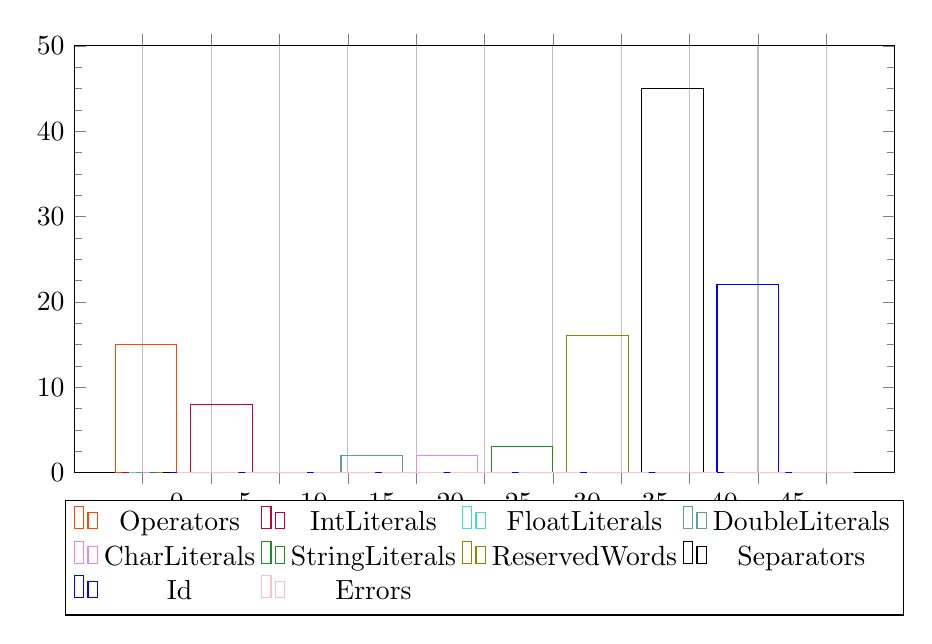
\begin{tikzpicture}
\begin{axis}[ybar interval, ymax=50,ymin=0, minor y tick num = 3, legend style={at={(0.5,-0.2)}, anchor=center, legend columns=4}, anchor=north, ybar interval=9,]
\addplot[color=OrangeRed] coordinates { (0, 15) (5, 0) (10, 0) (15, 0) (20, 0) (25, 0) (30, 0) (35, 0) (40, 0) (45, 0) (50, 0) };
\addplot[color=purple] coordinates { (0, 0) (5, 8) (10, 0) (15, 0) (20, 0) (25, 0) (30, 0) (35, 0) (40, 0) (45, 0) (50, 0)};
\addplot[color=Turquoise] coordinates { (0, 0) (5, 0) (10, 0) (15, 0) (20, 0) (25, 0) (30, 0) (35, 0) (40, 0) (45, 0) (50, 0)};
\addplot[color=CadetBlue] coordinates { (0, 0) (5, 0) (10, 0) (15, 2) (20, 0) (25, 0) (30, 0) (35, 0) (40, 0) (45, 0) (50, 0)};
\addplot[color=Violet] coordinates { (0, 0) (5, 0) (10, 0) (15, 0) (20, 2) (25, 0) (30, 0) (35, 0) (40, 0) (45, 0) (50, 0)};
\addplot[color=ForestGreen] coordinates { (0, 0) (5, 0) (10, 0) (15, 0) (20, 0) (25, 3) (30, 0) (35, 0) (40, 0) (45, 0) (50, 0)};
\addplot[color=olive] coordinates { (0, 0) (5, 0) (10, 0) (15, 0) (20, 0) (25, 0) (30, 16) (35, 0) (40, 0) (45, 0) (50, 0)};
\addplot[color=Black] coordinates { (0, 0) (5, 0) (10, 0) (15, 0) (20, 0) (25, 0) (30, 0) (35, 45) (40, 0) (45, 0) (50, 0)};
\addplot[color=blue] coordinates { (0, 0) (5, 0) (10, 0) (15, 0) (20, 0) (25, 0) (30, 0) (35, 0) (40, 22) (45, 0) (50, 0)};
\addplot[color=Pink] coordinates { (0, 0) (5, 0) (10, 0) (15, 0) (20, 0) (25, 0) (30, 0) (35, 0) (40, 0) (45, 0) (50, 1)};
\legend{Operators, IntLiterals, FloatLiterals, DoubleLiterals, CharLiterals, StringLiterals, ReservedWords, Separators, Id, Errors}
\end{axis}
\end{tikzpicture}
\end{frame}
\end{document}
